%%%%%%%%%%%%%%%%%%%%%%%%%%%%%%%%%%%%%%%%%%%%%%%%%%%%%%%%%%%%%%%%%%%%%%%%%%%%%%%%
%2345678901234567890123456789012345678901234567890123456789012345678901234567890
%        1         2         3         4         5         6         7         8

%\documentclass[letterpaper, 10 pt, conference]{ieeeconf}  % Comment this line out
% if you need a4paper
\documentclass[a4paper, 10pt, conference]{ieeeconf}      % Use this line for a4
% paper



% The following packages can be found on http:\\www.ctan.org
\usepackage{graphics} % for pdf, bitmapped graphics files
\usepackage{epsfig} % for postscript graphics files
%\usepackage{mathptmx} % assumes new font selection scheme installed
%\usepackage{times} % assumes new font selection scheme installed
%\usepackage{amsmath} % assumes amsmath package installed
%\usepackage{amssymb}  % assumes amsmath package installed

\title{\LARGE \bf
	Testing the Performance of Linear Regressors Using Inertial Information Combined with sEMG to Minimize the Limb Position Effect in Proportional and Simultaneous Control of Lower Arm Prosthetics.
}%final name

%\author{ \parbox{3 in}{\centering Huibert Kwakernaak*
%         \thanks{*Use the $\backslash$thanks command to put information here}\\
%         Faculty of Electrical Engineering, Mathematics and Computer Science\\
%         University of Twente\\
%         7500 AE Enschede, The Netherlands\\
%         {\tt\small h.kwakernaak@autsubmit.com}}
%         \hspace*{ 0.5 in}
%         \parbox{3 in}{ \centering Pradeep Misra**
%         \thanks{**The footnote marks may be inserted manually}\\
%        Department of Electrical Engineering \\
%         Wright State University\\
%         Dayton, OH 45435, USA\\
%         {\tt\small pmisra@cs.wright.edu}}
%}

\author{Simon Bruun, Oliver Thomsen Damsgaard, Martin Alexander Garenfeld, Irene Uriarte}% <-this % stops a space


\begin{document}
	
	
	
	\maketitle
	\thispagestyle{empty}
	\pagestyle{empty}
	
	
	%%%%%%%%%%%%%%%%%%%%%%%%%%%%%%%%%%%%%%%%%%%%%%%%%%%%%%%%%%%%%%%%%%%%%%%%%%%%%%%%
	\begin{abstract}
		Electromyography (EMG) is widely used for controlling functional prosthetics. However, EMG signals for the same movements change with variations in limb position and lowers the accuracy in control schemes \cite{fougner2012}. Most of the previous studies have utilized classification for pattern recognition when changing limb position, with a negative effect in performance. %Linear regression is a newer method in control of myoelectric prosthetics, which has proven to yield robust simultaneous and proportional control \cite{hanhe2014}. %Only the RMS feature was previously tested in variations of limb positions in regression-based control \cite{hwang2017}. 
This study investigated the effect of limb position in a linear regression-based control scheme, when using 
%the commonly used 
Mean Absolute Value (MAV) and Logarithmic Variance (LogVar) as features. %where the latter has shown linear properties \cite{hanhe2014}.
Seven (more now) able-bodied subjects were recruited for data acquisition, performing four wrist movements in three different limb positions. One regression model was build to recognize the different wrist movements under study, taking into account both features. %One regression model %(regressor) 
%was build for each wrist movement for each test subject: four for each feature. 
The regressors were tested online in a virtual environment. %where the time to complete a target-reaching task of sixteen targets was measured. %The performance (time per reached target) of the online test was compared between the different limb positions of the same feature and between all limb positions of the two features through statistical analysis. 
%Using a Friedman's test the performance scores between the three limb positions prove not to be significantly different 
%(p = 0.5647), 
%when applying the LogVar trained regressors %in the online test. For the MAV trained regressors the performance score between all limb positions cannot be proven significantly different either (p = 0.1561). 
%There was no difference in the time to reach the targets across the two features %(LogVar: 6.5 s, MAV: 5.5 s; p = 0.13).
The results showed that changes in limb position do not affect the control when linear regression model is trained with the %MAV or LogVar 
features extracted. This is opposed to previous studies using classification as control scheme. Linear regression has the potential to be used in future control schemes for myoelectric prosthetics for use in daily life tasks.\\


\textit{\textbf{Keywords---}}surface electromyography, inertial measurement unit, simultaneous and proportional myoelectric control, regression, hand motion classification, hand prosthetic


	\end{abstract}
	
	
	%%%%%%%%%%%%%%%%%%%%%%%%%%%%%%%%%%%%%%%%%%%%%%%%%%%%%%%%%%%%%%%%%%%%%%%%%%%%%%%%
	\section{INTRODUCTION}
		
		%What has been done in the EMG-prosthesis area?
In recent years the development of EMG controlled lower arm prosthetics has advanced considerably, due to an increased interest in the area along with higher demands for better prosthetics and more precise control. \cite{Fougner2012} In the early years most EMG prosthetics functioned by controlling one degree of freedom (DOF) with on-off control, mainly by linking antagonistic muscles to one DOF. This kind of prostheses change between states due to a switching impulse which cause a state machine to shift its present state. Usually a strong and fast muscle contraction from the users is employed to generate the switching signals. \cite{amsuess2014}
This type of control provided users a way to control more than one DOF, but never simultaneously. The switch-control functioned on a cycle, so users would have to go through all the movements of the prosthesis to find the one they wanted to perform. However, as demands rose, more complex methods was introduced to the EMG prosthetics scene. Classification methods effectively enabled users to use DOF's more freely because the switching was now replaced by direct recognition of different muscle contractions linked to specific prosthetic movements. This also effectively enabled proportional control of movements, but gave rise to new problems: a wider range of control would give less accurate movements, and training the classifiers proved difficult, as the training could over-fit, causing extended use of the prosthetics to degrade in performance. \cite{Ison2016}

%Regression
Introducing regression as a new mapping method in myoelectric prosthetics provided a way to enable both simultaneous and proportional control of multiple DOF's. Regression is able to provide a continuous value for each DOF based on the recorded EMG signal, while a classifier only decides upon a certain class. \cite{hahne2014, jiang2010}
This means that classification can only translate a recorded EMG signal to one movement of the prosthetic at a time. It can do so proportionally but the handling still lacks natural control, since movements by able-bodied individuals very rarely only happen in one DOF at a time. Regression methods constantly provide a value, and since several regressors can be used at a time, several values can be used in the recognition of movements. This is what enables regression methods to perform simultaneous and proportionally. 

Applying regression as a mapping method in proportional and simultaneous control of multiple DOF's has been shown to perform well in recognition of movements and doing so with a low computation time. \cite{hahne2014} However, very few studies have tested the regressor performance in daily life tasks outside the clinical training environment. \cite{jiang2012} A study by Fougner et al. \cite{Fougner2011} has addressed the problem that most studies test their method on only one limb position. This means that the actual performance of regression methods has not yet been properly addressed when recognizing movements, where the arm changes position during daily life tasks. 

%Which issues are there in the EMG-prosthesis area?(decreasing quality of control of hand gestures when the arm is placed in different positions)
When recording EMG signals it has been shown that some muscles are activated based on joint angles, even though the muscles are not involved in the movement of that joint \cite{Fougner2011}. This provides a problem, but can be explained by muscle-synergies \cite{DeRugy2013}. These muscle-synergies are created by the Central Nervous System (CNS) and coordinated into activation of different muscles at varying times. This enables the CNS to control the muscle-synergies instead of controlling each muscle individually to perform movements \cite{jiang2009}. This means that muscles in the lower arm can be activated when muscles in the upper arm are activated, in a level that will be detectable in EMG recordings, and enough to alter recognition of movements, when the arm is active in limb positions other than those tested in a clinical environment. 

%What would be novel to add to this area?(adding IMU’s to a regressor, since it has been done with a classifier)
In order to overcome the problem of muscles-synergies, Fougner et al. \cite{Fougner2011} has suggested to combine recordings of EMG signals with inertial information to provide limb position data. This could be beneficial in increasing the accuracy of EMG controlled prosthetics for use in daily life tasks. 
Even though the combination of EMG and Inertial Measurement Unit (IMU) data has been proposed as a valid way to improve the performance and accuracy of EMG based prosthetics, it has only been investigated in few studies. \cite{Roy2010, Imtiaz2014, jiang2012}

To the authors knowledge the combination of EMG recordings and IMU data has only been done with classification methods. A novel approach to further investigate the usability of combining EMG and IMU is to build a regression based control scheme for myoelectric prosthetics. This would enable both proportional and simultaneous control of several DOF's, where the inclusion of IMU data should provide more information on limb position to counter the effect of limb position.






%In recent years the development of EMG controlled prosthesis have advanced due to an increased interest in the area as well as a higher demand of better control of this prosthesis.\cite{fougner2012}
%In the early years most EMG prosthetics functioned by only controlling one DOF by \textit{on-off control}, mostly by linking antagonistic muscles to one DOF. %This along with \textit{mode switching} provided users a way to control more than one DOF, but not in a simultaneous way. 
%This control provided a way to control more than one DOF, but not simultaneously. However, as demands would rise, more complex methods were introduced to the EMG scene. Classification methods enabled simultaneous control of more than one DOF, but gave rise to new problems; a wider range of control would give less accurate movements, and training the pattern recognition methods proved difficult, as the training could over-fit, causing extended use of the prosthetics to degrade in performance. \cite{Ison2016}.
% 
%It has been proved that regression techniques can be apply as a new mapping method to achieve simultaneous and proportional control of multiple DOFs\cite{hanhe2014}. Regression methods provide a continous value for each DOF based on the recorded EMG signal, while classification methods only decides upon a certain class. However there are still difficulties when prosthesis perform outside the clinical training environment\cite{jiang2012}.
% Fougner et al.\cite{Fougner2011} noticed that majority of studies only take in account one limb position. It has been shown that some muscles are activated based on joint angles \cite{reference}, even though the muscles are not involved in the movement of that joint, which can be explained by muscle-synergies existed between muscles.
%% which becomes a problem since muscles create muscle-synergies to perform movements. 
%Variations in limb positions can have an impact on the robustness of EMG pattern recognition. %To be able to offer a good perform of the prosthesis, these should be able to execute with the same accuracy diverse hand gestures in different limb positions. 
%In order to overcome this problem it has been suggested to combine EMG data as well as IMU data, to provide limb position information. Nevertheless this combination of data have only been investigated for classification methods. 
%In this study we test the performance of linear regression methods combining EMG and IMU data for a simultaneous and proportional control of two DOFs in a lower-arm prothesis while the arm is located in different limb positions.
%% in the training sesions of the regressor to obtain simultaneous and proportional control of EMG prosthesis. 
%%Hypotheses
%%Simultaneous and proportional control of two  DOF's of the wrist in different limb positions, can be achieve trough the use of linear regression as control system. Combining EMG and IMU's can minimize the limb position effect when using regression as control system.
	
	\section{METHODS}
	
		\subsection{Experimental Setup}
EMG data was collected from (define number) able-bodied subjects. The subjects performed four different hand gestures. This study is only focus on two DOF, which are, flexion, extension, radial and ulnar deviation of the wrist. The order in the execution of the movements was the same for each subject. EMG signals were recorded with Myo armband, positioned in the right forearm of the subjects (all subjects right handed). The procedure was performed in three different limb positions. In order to avoid shoulder fatigue a relaxation period was given between trials. The subjects were instructed not to move the fingers during the data acquisition. The process was performed in a standing position. \\ %figure hand and limb positions
 Myo armband counts with eight medical grade stainless steel surface EMG sensors. %It is capable of pulling EMG data at a sample rate of 200 Hz. 
 Furthermore its nine axis IMU provides information about position and orientation of the arm combining three axis accelerometer, three axis gyroscope and three axis magnetometer.\\   
 In order to acquire the training data necessary to build the regressor, a graphical user interface (GUI) was implemented in MATLAB. %Firstly baseline was meassure holding the forearm relaxed and the wrist in a neutral position for the corresponding limb position. This measure was substracted from the signal afterwards to be able to remove the present artefacts. Subsequently maximum voluntary contraction (MVC) was meassure. The MVC  was calculated as a mean of the maximum values in each of the eight cannels, and was set as a normalized reference point of 1.
 %The data acquisition was depicted through a trapeze. MVC was set as the desired value before data acquisition. Consequently each hand gesture was performed as a fraction of the MVC. At the begining of the training data collection two second resting phase was given followed by two seconds ascending slope to reach the plateau phase, with a duration of three seconds. Afterwards a descending phase of two seconds and a resting phase of one second finalized the data acquisition. The total acquisition time was ten seconds per hand movement.

	%\subsection{Maintaining the Integrity of the Specifications}
	
	%The template is used to format your paper and style the text. All margins, column widths, line spaces, and text fonts are prescribed; please do not alter them. You may note peculiarities. For example, the head margin in this template measures proportionately more than is customary. This measurement and others are deliberate, using specifications that anticipate your paper as one part of the entire proceedings, and not as an independent document. Please do not revise any of the current designations
	
	\subsection{Preprocessing}
	For this study the EMG data acquired were filtered using a second-order Butterworth high-pass filter, cutoff frequency ($f_c$=10Hz), to avoid low frequency movement artefacts in the recorded signal.\\
	%review two states part trapeze!!
	%The EMG signal is the result of the addition of different motor unit action potential trains (MUAPTs). Through the data acquisition phase EMG signal can be divided into two main states. The transient state, related with the beginning phase of the muscle contraction and the steady state which is the stable phase of the muscle contraction when a constant position is held \cite{mobarak2014}. Although the steady state only contains a short temporal structure of the patterns involved in the contraction of the muscle \cite{mobarakm2014}, studies has shown that it is possible to achieve online continuous control using steady state EMG signals.This could be due to the fact that a larger amount of meaningful data is contained in this muscle contraction phase \cite{mobarakm2014}. For the training of the control system in this project the steady signal was then used.
	
	\subsection{Feature extraction}
	The features were extracted creating a sliding-window of 40 samples. % with an overlapping of the 50\%. 
	Two different time domain features were extracted, MAV as well as LogVar. MAV represent the amplitud of the signal. It is defined as the average of the absolute values of the EMG signal and expresed as:
	\begin{equation}
	MAV = \frac{1}{N}\sum\limits_{i=1}^N|x_i|
	\end{equation}
	where N is the length of the signal, and $x_i$ is the signal of $i$ samples.
	The LogVar is a nonlinear transformation of the variance, which has been shown to behaves more linear than other time domain features. \cite{hanhe2014}
	\begin{equation} \label{eq:logvar}
	log(\sigma^2) = log(\frac{\sum\limits_{i=1}^N(x_i - \mu)^2}{N})
	\end{equation}
	where N expresses the length of the signal, $x_i$ is the $i^th$ sample of the signal and $\mu$ is the mean.
	\subsection{Separability of data}
Principal Component Analysis (PCA) was applied to be able to evaluate the quality of the features extracted from the EMG signals.
	%This analysis tool express a set of correlated variables into non-correlated components. In that way, the data set can be expressed in a reduced dimensionality hyperspace using less but most representative variables which are the principal components. Through PCA is  possible to see significant outliers or if the clusters formed by the features can be easily distinguishable. This was done to avoid inaccurate training of the regressors. PCA was performed for each movement in each limb position. %and represented in three dimensional space.figure? 
	\subsection{Data exclusion}
	Some of the subjects were not able to perform through the study properly. In order to ensure constant data those subjects were exclude.
	\subsection{Regression models}
	The acquired data was used to built the different regressors that had been implemented, one for each movement under study and for both features. Multivariate linear regression as an extension of simple linear regression had been applied as is shown in \ref{reg}:
\begin{equation}
	\hat{Y} = \alpha + \beta_1 X_{1} + \beta_2 X_{2} + ... + \beta_i X_{i} + \epsilon_i
		\label{reg}
\end{equation}
	where $Y$ is the dependent variable, $X_i$ are the independent variables, $\beta_i$ is the regression coefficient in the sampled population, $\alpha$ is the predicted value of $Y$ at $X = 0$ and $\epsilon$ is the error.
	
	\subsection{Regressor accuracy}
	Superimposition\\
	In order to examine the performance of the regressors the estimations of the regressor and the actual data for the two different features extracted had been superimposed. Thereby the behave of the regressor can be shown at different intensities and movements. Consequently whether other regression methods should be considered to obtain a lower error.\\
	RMSE\\
	To meassure the accuracy of the regressor, Root Mean Squared Error (RMSE) was calculated. RMSE is a calculation of the standard deviation of the residuals, that is, the difference between the estimated and the actual values.
	%equation
	\begin{equation}
	RMSE = \sqrt{\frac{\sum\limits_{i=1}^N(y_i - \hat{y_i})^2}{N}}
	\end{equation}
	Where N is the length of the signal, $y_i$ is the $i^th$ variable of the actual data and $\hat{y_i}$ is the $i^th$ output of the regressor. The RMSE will be done for the regressor of each movement.\\
	
	%Fitts Law\\
	%A modified version of Fitts' Law had been used to quantify the performance of the trained regressors. Fitts' Law describes that, the time it takes to do a rapid movement to reach a target area, is dependent on the distance to the target area, and the size of the target area. The law demonstrates that the information of any human motor tasks, is finite and only limited by the capabilities of the control system. The control exhibit a negative correlation between speed and accuracy. \cite{Kamavuako2014}
	%Fitts' Law calculates an \textit{Index of Difficulty} (ID) by \ref{eq:Fitts}
	
%	\begin{equation} \label{eq:Fitts}
	%ID = log_{2} \cdot (\frac{2D}{W})
	%\end{equation}
	
	%where D is distance to the targets and W is width of target area. The system in this study does not provide a reasonable scale for distance and target width, for this reason Fitts' Law cannot be apply as usual. Instead, the time it takes a subject to reach the targets as well as the number of targets reached will be noted to calculate a performance score as shown in \ref{eq:ourScore}.
	
	%\begin{equation} \label{eq:ourScore}
	%Score = \frac{time}{targets\ reached}
	%\end{equation}
	%Consequently low score results represent the best performance.
	%To accomplish the modified Fitts' Law test a compass-plot was implemented in the GUI Fig.\ref{figurelabel}. The subjects had to reach 16 targets distributed around the origin in two different radius. This allows to test the proportional control. The targets were fixed in the diagonals of the compass-plot to be able to test simultaneous control. The amount of targets reached in each quadrant gives important information about the regressor performance as well as, providing the weak directions.
	
	
	

	
	\section{RESULTS}
	
			\begin{figure}[!thpb]
		\centering
		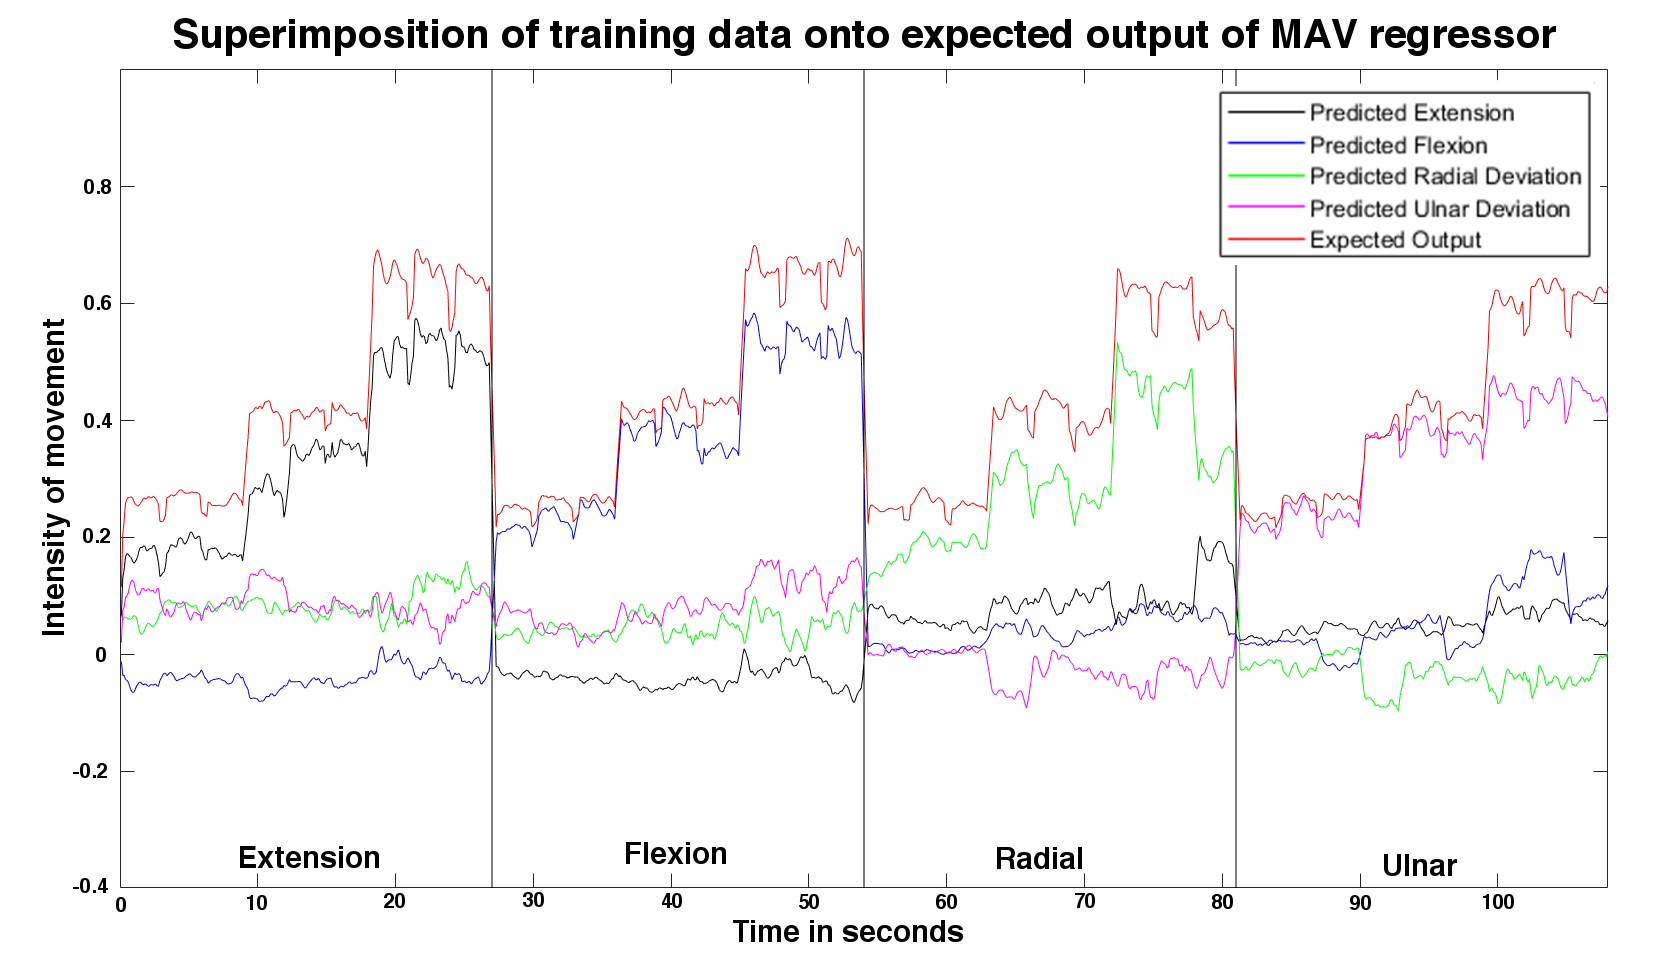
\includegraphics[width=0.4\textwidth]{figures/NewSuperPositionTestDataMAV}  %<--but is not needed.
		\caption{Plot of the actual data, red plot, superimposed on the output of the regressors trained with the MAV features. The plot is divided into four segments, where each segment shows a different movement performed. Each segment has the same sample size.}
		\label{fig:SuperPositionTrainingMAV}  %<--give the figure a label, so you can reference!
	\end{figure}
	
	\begin{figure}[!thpb]
		\centering
		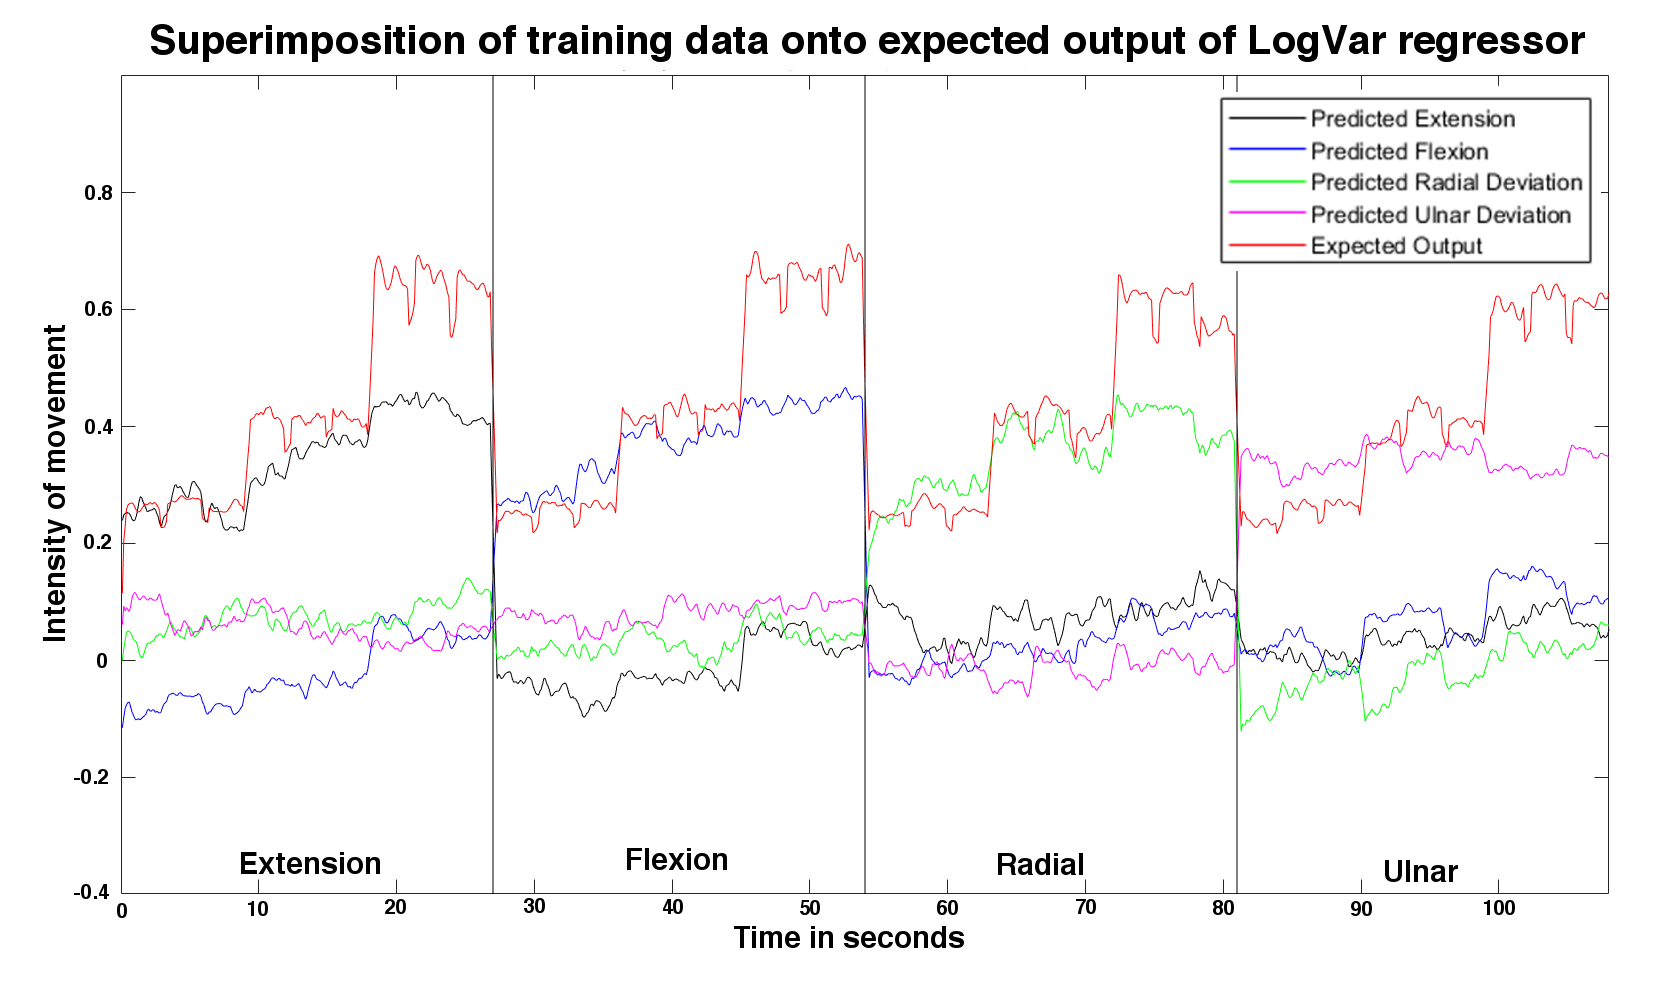
\includegraphics[width=0.4\textwidth]{figures/NewSuperPositionTestDataLogVar}  %<--but is not needed.
		\caption{Plot of the actual data, red plot, superimposed on the output of the regressors trained with the LogVar features. The plot is divided into four segments, where each segment shows a different movement performed. Each segment has the same sample size.}
		\label{fig:SuperPositionTrainingLogVar}  %<--give the figure a label, so you can reference!
	\end{figure}
	
	\begin{table}[!thpb]
		\begin{center}
			\begin{tabular}{l l l}
				\hline
				\textbf{Feature} & \textbf{Overall mean error} & \textbf{Standard deviation}\\
				\hline
				Extension & 0.1030 & $\pm 0.0210$ \\
				Flexion & 0.1102 & $\pm 0.0296$ \\
				Radial Deviation & 0.1206 & $\pm 0.0298$ \\
				Ulnar Deviation & 0.1143 & $\pm 0.0334$ \\
				Overall & 0.1059 & $\pm 0.0306$ \\
				\hline
			\end{tabular}
			\caption{RMSE for the implemented MAV regressor}
		\end{center}
	\end{table}
	
	\begin{table}[!thpb]
		\begin{center}
			\begin{tabular}{l l l}
				\hline
				\textbf{Feature} & \textbf{Overall mean error} & \textbf{Standard deviation}\\
				\hline
				Extension & 0.1157 & $\pm 0.0469$ \\
				Flexion & 0.1102 & $\pm 0.0241$ \\
				Radial Deviation & 0.1142 & $\pm 0.0256$ \\
				Ulnar Deviation & 0.1312 & $\pm 0.0310$ \\
				Overall & 0.1178 & $\pm 0.0272$ \\
				\hline
			\end{tabular}
			\caption{RMSE for the implemented LogVar regressor}
		\end{center}
	\end{table}
	
	\begin{table}[!thpb]
		\begin{center}
			\begin{tabular}{l l l}
				\hline
				\textbf{Feature} & \textbf{Overall mean error} & \textbf{Standard deviation}\\
				\hline
				Extension & 0.1646 & $\pm 0.0753$ \\
				Flexion & 0.1391 & $\pm 0.0841$ \\
				Radial Deviation & 0.2018 & $\pm 0.0424$ \\
				Ulnar Deviation & 0.1743 & $\pm 0.0905$ \\
				Overall & 0.1700 & $\pm 0.0759$ \\
				\hline
			\end{tabular}
			\caption{RMSE for the implemented MAV regressor}
		\end{center}
	\end{table}
	
	The overall mean of the RMSE of MAV is 0.0943 with a standard deviation of $\pm 0.0290$, where the highest mean of a regressor is 0.1088 and the highest standard deviation is $\pm 0.0366$. The overall mean of the RMSE of LogVar is 0.1107 with a standard deviation of $\pm 0.0298$, where the highest mean of a regressor is 0.1216 and the highest standard deviation is $\pm 0.0402$. MAV appears to yield a lower mean RMSE and a lower standard deviation than LogVar - both with the overall RMSE and for the movement with the highest RMSE.
	
	\begin{table}[!thpb]
		\begin{center}
			\begin{tabular}{l l l}
				\hline
				\textbf{Feature} & \textbf{Overall mean error} & \textbf{Standard deviation}\\
				\hline
				Extension & 0.1552 & $\pm 0.0514$ \\
				Flexion & 0.1680 & $\pm 0.0508$ \\
				Radial Deviation & 0.1681 & $\pm 0.0540$ \\
				Ulnar Deviation & 0.2078 & $\pm 0.0621$ \\
				Overall & 0.1748 & $\pm 0.0563$ \\
				\hline
			\end{tabular}
			\caption{RMSE for the implemented LogVar regressor}
		\end{center}
	\end{table}
	
	\begin{table}[!thpb]
		\begin{center}
			\begin{tabular}{l l}
				\hline
				\textbf{Compared features} & \textbf{P-Value}\\
				\hline
				LogVar, MAV & 0.0044 \\
				LogVar test data, MAV test data & 0.1138 \\
				LogVar test data, LogVar & 0.0001 \\
				MAV test data, MAV & 0.000002 \\
				\hline
			\end{tabular}
			\caption{P-Values for comparison of the features}
		\end{center}
	\end{table}
	It was found that the P-value of a Friedman's statistical test showed a significant difference (p = 0.0044) between the RMSE for the MAV and LogVar regressors with the training data as input, where LogVar has the higher mean. When examining the RMSE for the regressors with unknown test data consisting of 50\% contractions of all movements in all limb positions, it was shown that there is no significant difference (p = 0.1138) between the offline performance of the two regressors. When comparing the offline tests with training data and 50\% test data, it was shown that there's a significant difference for both LogVar (p = 0.000002) and LogVar (p = 0.0001), where the mean is higher for the unknown 50\% data in both cases.
	
	\begin{figure}[!thpb]
		\centering
		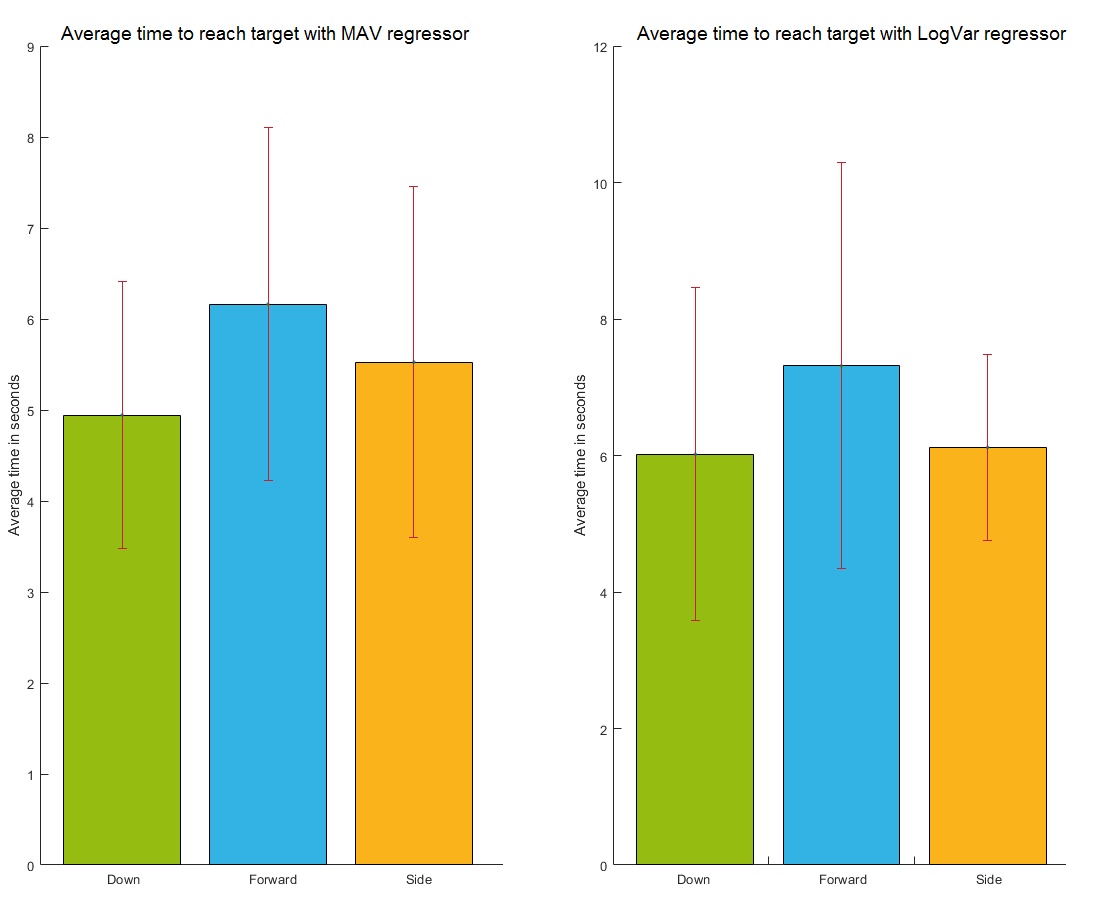
\includegraphics[width=0.4\textwidth]{figures/GotItTime}  %<--but is not needed.
		\caption{Plot of the actual data, red plot, superimposed on the output of the regressors trained with the MAV features. The plot is divided into four segments, where each segment shows a different movement performed. Each segment has the same sample size.}
		\label{fig:GotItTime}  %<--give the figure a label, so you can reference!
	\end{figure}
	
	\begin{table}![thpb]
		\begin{center}
			\begin{tabular}{l l l}
				\hline
				\textbf{Limb position, feature} & \textbf{Overall mean error} & \textbf{Standard deviation}\\
				\hline
				Down, MAV & 5.3377 & $\pm 1.5696$ \\
				Forward, MAV & 8.1791 & $\pm 4.7145$ \\
				Side, MAV & 6.0490 & $\pm 2.0490$ \\
				Down, LogVar & 6.5404 & $\pm 2.5315$ \\
				Forward, LogVar & 7.9123 & $\pm 3.4572$ \\
				Side, LogVar & 6.9325 & $\pm 2.3036$ \\
				\hline
			\end{tabular}
			\caption{Test scores for the different limb for MAV and LogVar regressors}
		\end{center}
	\end{table}
	\begin{table}[!thpb]
		\begin{center}
			\begin{tabular}{l l}
				\hline
				\textbf{Feature} & \textbf{P-Value}\\
				\hline
				MAV & 0.8948 \\
				LogVar & 0.2359 \\
				\hline
			\end{tabular}
			\caption{P-Values for comparison of the score in different limb positions with MAV and LogVar}
		\end{center}
	\end{table}
	
	A one-sample Kolmogorov-Smirnov test was done on the scores from the MAV and LogVar respectively and showed no normality in both score sets(p = $7 * 10^{-20}$, $8 * 10^{-20}$ ). A Friedman's test was therefore applied for statistical analysis. The performance scores between the three limb positions prove not to be significantly different (p = 0.2359), when applying the LogVar trained regressors in the online test. For the MAV trained regressors the performance score between all limb positions can not be proven significantly different either (p = 0.8948). 
	
	\begin{table}[!thpb]
		\begin{center}
			\begin{tabular}{l l l}
				\hline
				\textbf{Limb position, feature} & \textbf{Overall mean error} & \textbf{Standard deviation}\\
				\hline
				Down, MAV & 15.5556 & $\pm 0.7265$ \\
				Forward, MAV & 15.1111 & $\pm 1.0541$ \\
				Side, MAV & 15.2222 & $\pm 0.8333$ \\
				Down, LogVar & 15.4444 & $\pm 0.7265$ \\
				Forward, LogVar & 15 & $\pm 1.8020$ \\
				Side, LogVar & 15.3333 & $\pm 1.1180$ \\
				\hline
			\end{tabular}
			\caption{Targets reached in the target test with the MAV and LogVar regressors.}
		\end{center}
	\end{table}
	
	\begin{table}[!thpb]
		\begin{center}
			\begin{tabular}{l l}
				\hline
				\textbf{Feature} & \textbf{P-Value}\\
				\hline
				MAV & 0.0212 \\
				LogVar & 0.4220 \\
				\hline
			\end{tabular}
			\caption{P-Values for comparison of the number of reached targets in different limb positions with MAV and LogVar}
		\end{center}
	\end{table}
	
	The Friedman's statistical test shows a significant difference (p = 0.0212) between the number of targets reached in the different limb positions for the MAV regressor, where the worst performance was found when the test subjects pointed their arm forward (mean = 15.1111). There was no significant difference (p = 0.4220) between the limb positions for the LogVar regressor.
	
	\begin{figure}[!thpb]
		\centering
		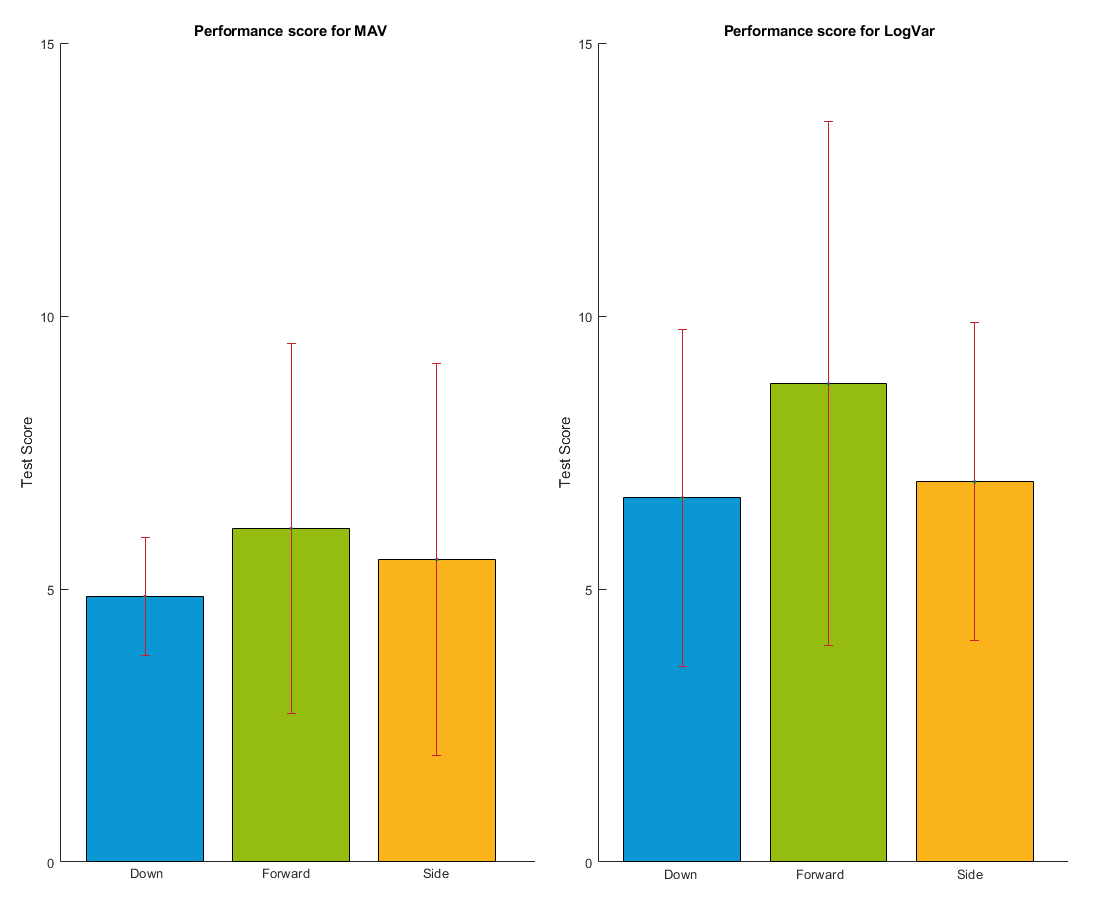
\includegraphics[width=0.4\textwidth]{figures/GotItTimeIMU}  %<--but is not needed.
		\caption{Plot of the actual data, red plot, superimposed on the output of the regressors trained with the MAV features. The plot is divided into four segments, where each segment shows a different movement performed. Each segment has the same sample size.}
		\label{fig:GotItTimeIMU}  %<--give the figure a label, so you can reference!
	\end{figure}
	
	\begin{table}[!thpb]
		\begin{center}
			\begin{tabular}{l l l}
				\hline
				\textbf{Limb position,feature} & \textbf{Overall mean error} & \textbf{Standard deviation}\\
				\hline
				Down, MAV & 4.8661 & $\pm 1.0839$ \\
				Forward, MAV & 6.1094 & $\pm 3.3852$ \\
				Side, MAV & 5.5442 & $\pm 3.5847$ \\
				Down, LogVar & 6.6691 & $\pm 3.0798$ \\
				Forward, LogVar & 8.7595 & $\pm 4.7969$ \\
				Side, LogVar & 6.9652 & $\pm 2.9144$ \\
				\hline
			\end{tabular}
			\caption{Test scores for the different limb for MAV and LogVar regressors with IMU included.}
		\end{center}
	\end{table}
	
	\begin{table}[!thpb]	
		\begin{center}
			\begin{tabular}{l l}
				\hline
				\textbf{Feature} & \textbf{P-Value}\\
				\hline
				MAV & 0.0319 \\
				LogVar & 0.4594 \\
				\hline
			\end{tabular}
			\caption{P-Values for comparison of the score in different limb positions with MAV and LogVar with IMU data included}
		\end{center}
	\end{table}
	
	The test with IMU data included shows a significant difference (p = 0.0319) between the test score in different limb positions for the MAV regressor with the worst performing position was with the arm pointed forward (mean = 6.1094), while there is no difference proven in the LogVar test (p = 0.4594).
	
	\begin{table}[!thpb]
		\begin{center}
			\begin{tabular}{l l l}
				\hline
				\textbf{Limb position,feature} & \textbf{Overall mean error} & \textbf{Standard deviation}\\
				\hline
				Down, MAV & 15.8889 & $\pm 0.3333$ \\
				Forward, MAV & 15.1111 & $\pm 2.3154$ \\
				Side, MAV & 15.5556 & $\pm 1.3333$ \\
				Down, LogVar & 14.7778 & $\pm 1.7159$ \\
				Forward, LogVar & 13.5556 & $\pm 2.1858$ \\
				Side, LogVar & 14.1111 & $\pm 1.8333$ \\
				\hline
			\end{tabular}
			\caption{RMSE for the implemented LogVar regressor}
		\end{center}
	\end{table}
	
	\begin{table}[!thpb]
		\begin{center}
			\begin{tabular}{l l}
				\hline
				\textbf{Compared Features} & \textbf{P-Value}\\
				\hline
				MAV & 0.2957 \\
				LogVar & 0.0037 \\
				\hline
			\end{tabular}
			\caption{P-Values for comparison of the number of targets reached in different limb positions with MAV and LogVar with IMU data included}
		\end{center}
	\end{table}
	
	The number of targets reached in the different limb positions can be proven to be significantly different (p = 0.0037) for the LogVar feature with IMU data included, where the lowest number of targets reached (mean = 13.5556) was found when the subjects pointed their arm forward. There was no significant difference found for the MAV regressor with IMU data included (p = 0.2957).
	
	\begin{figure}[!thpb]
		\centering
		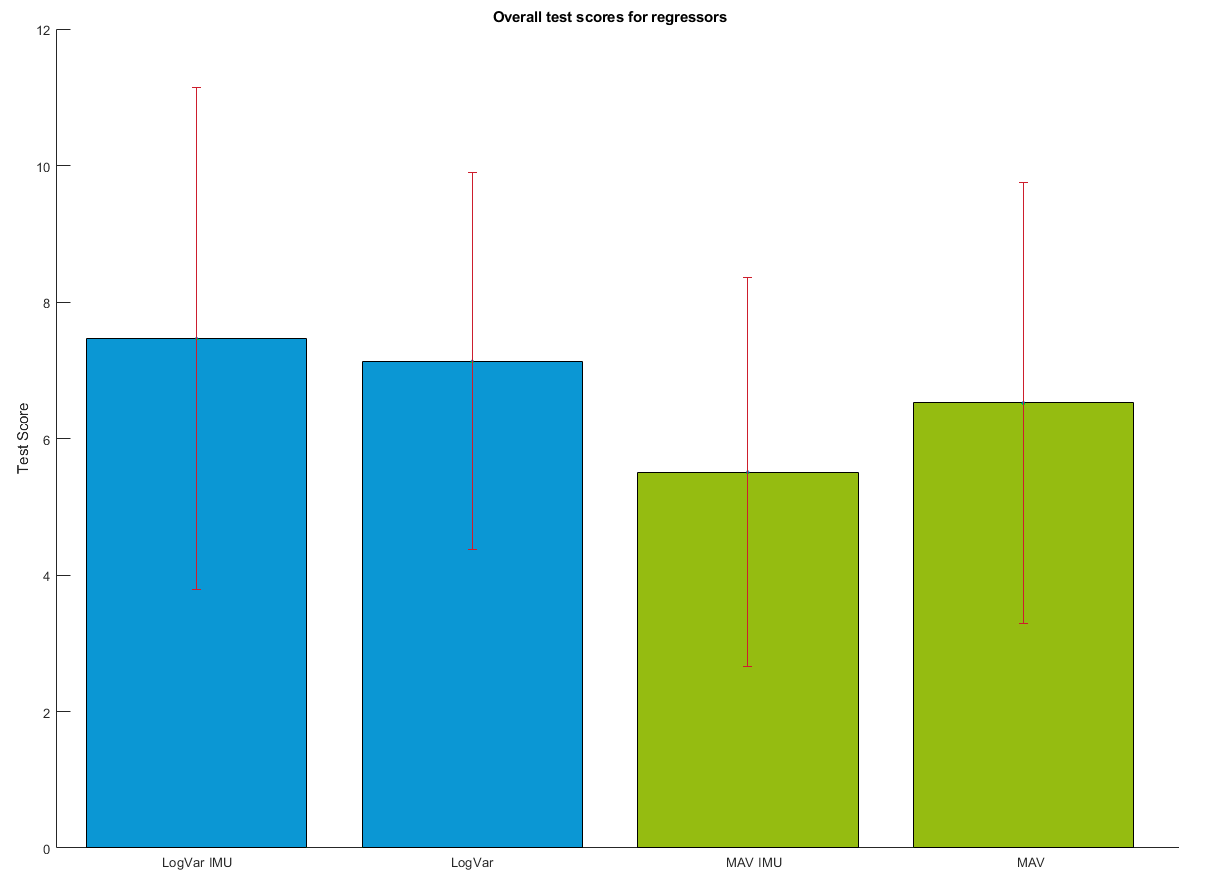
\includegraphics[width=0.4\textwidth]{figures/allRegressorBarzTimeScoreForTargetTest}  %<--but is not needed.
		\caption{Plot of the actual data, red plot, superimposed on the output of the regressors trained with the MAV features. The plot is divided into four segments, where each segment shows a different movement performed. Each segment has the same sample size.}
		\label{fig:TimeScoreTargets}  %<--give the figure a label, so you can reference!
	\end{figure}
	
	\begin{table}[!thpb]
		\begin{center}
			\begin{tabular}{l l l}
				\hline
				\textbf{Feature} & \textbf{Mean score} & \textbf{Standard deviation}\\
				\hline
				MAV & 6.5219 & $\pm 3.2253$ \\
				MAV w. IMU & 5.5066 & $\pm 2.8477$ \\
				LogVar & 7.1284 & $\pm 2.7619$ \\
				LogVar w. IMU & 7.4646 & $\pm 3.6740$ \\
				\hline
			\end{tabular}
			\caption{Average score of the target test for the four regressor designs}
		\end{center}
	\end{table}
	
	\begin{table}[!thpb]
		\begin{center}
			\begin{tabular}{l l}
				\hline
				\textbf{Compared features} & \textbf{P-Value}\\
				\hline
				LogVar w/ IMU, MAV w/ IMU & 0.5637 \\
				LogVar, MAV & 0.0833 \\
				LogVar w/ IMU, LogVar & 0.5637 \\
				MAV w/ IMU, MAV & 0.1779 \\
				\hline
			\end{tabular}
			\caption{P-Values for comparison of the overall scores of the target tests}
		\end{center}
	\end{table}
	
	When comparing all performance scores from the two feature trained regression control schemes without IMU, the Friedman's test proves no significant difference (LogVar: 7.1284 s, MAV: 6.5219 s; p = 0.0833). There is no significant difference to be found between LogVar and MAV with IMU data included (LogVar w/ IMU: 7.4646, MAV w/ IMU: 5.5066, p = 0.5637), and no difference was found between features with and without IMU for either MAV (w/o IMU: 6.5219, w/ IMU: 5.5066, p = 0.1779) or LogVar (w/o IMU: 7.1284, w/ IMU: 7.4646, p = 0.5637).
	
	\begin{figure}[!thpb]
		\centering
		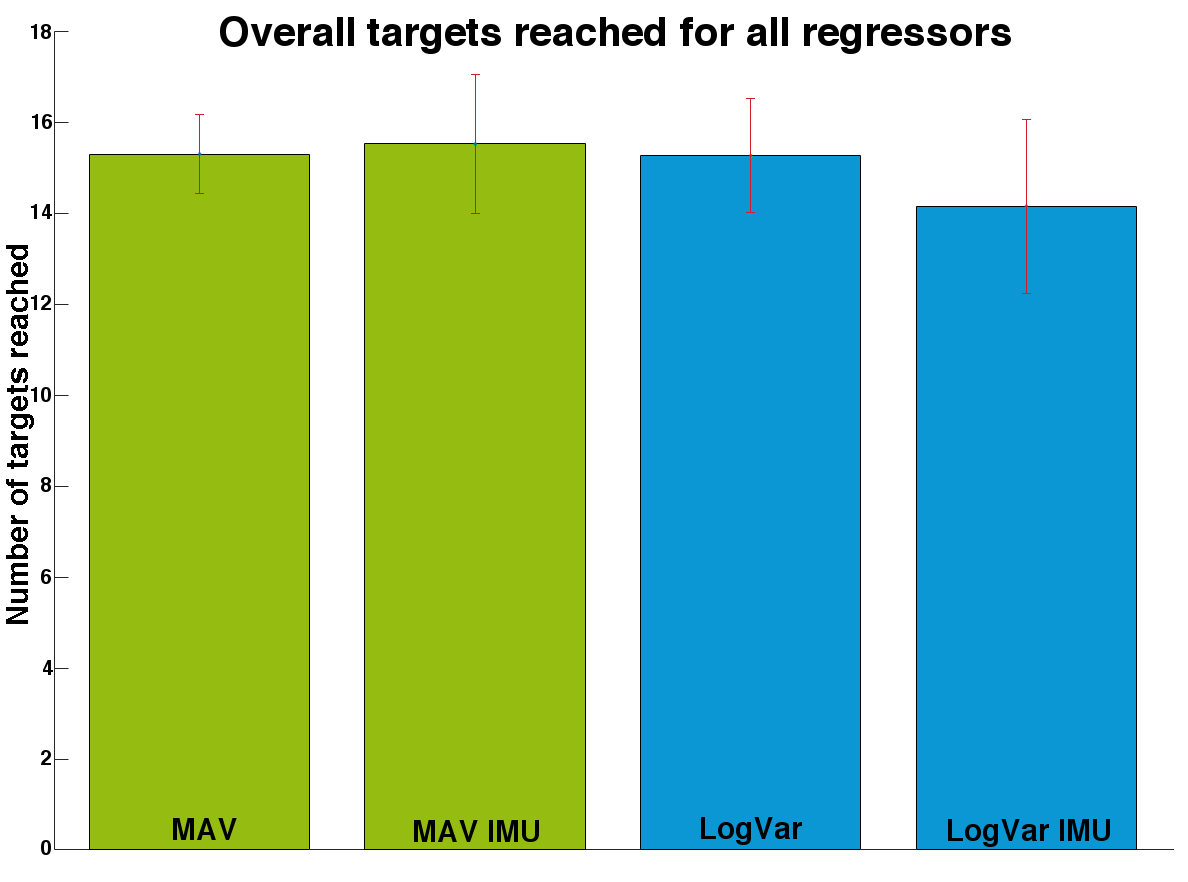
\includegraphics[width=0.4\textwidth]{figures/sumMoreBarsWithTargetsReachedForAllRegressors}  %<--but is not needed.
		\caption{Plot of the actual data, red plot, superimposed on the output of the regressors trained with the MAV features. The plot is divided into four segments, where each segment shows a different movement performed. Each segment has the same sample size.}
		\label{fig:TargetScoresTargets}  %<--give the figure a label, so you can reference!
	\end{figure}	
	
	\begin{table}[!thpb]
		\begin{center}
			\begin{tabular}{l l l}
				\hline
				\textbf{Feature} & \textbf{Overall mean error} & \textbf{Standard deviation}\\
				\hline
				MAV & 15.2963 & $\pm 0.8689$ \\
				MAV w/ IMU & 15.5185 & $\pm 1.5285$ \\
				LogVar & 15.2593 & $\pm 1.2586$ \\
				LogVar w/ IMU & 14.1481 & $\pm 1.9156$ \\
				\hline
			\end{tabular}
			\caption{Average number of targets reached in the target test for the four regressor designs}
		\end{center}
	\end{table}
	
	\begin{table}[!thpb]
		\begin{center}
			\begin{tabular}{l l}
				\hline
				\textbf{Compared Features} & \textbf{P-Value}\\
				\hline
				LogVar w/ IMU, MAV w/ IMU & 0.0017 \\
				LogVar, MAV & 1 \\
				LogVar w/ IMU, LogVar & 0.0016 \\
				MAV w/ IMU, MAV & 0.0124 \\
				\hline
			\end{tabular}
			\caption{P-Values for comparison targets reached in the target tests}
		\end{center}
	\end{table}
	
	A significant difference was found between LogVar and MAV when IMU was included (LogVar w/ IMU: 14.1481, MAV w/ IMU: 15.5185, p = 0.0017), and the same was found when including IMU data for both MAV (w/o IMU: 15.2963, w/ IMU: 15.5185, p = 0.0124) and LogVar (w/o IMU: 15.2593, w/ IMU: 14.1481, p = 0.0016). The performance was similar when comparing the overall number of targets reached for LogVar and MAV (p = 1).
	
	
	%	\subsection{Separability of the data} 
	
	
	
	%PCA performance for both features extracted is illustrated in Fig. \ref{PCA_MVA} (MVA) and in Fig. \ref{PCA_logvar} (logarithmic variance).
	%The importance of each component for MAV and logarithmic variance is represented in Fig. \ref{PCA_MVA}(a) and Fig. \ref{PCA_logvar}(a) respectively. On the one hand for the MAV feature making use of the three first components, 93.8\% of the data set can be described. On the other hand for the logarithmic variance feature the 93.97\% of the data set is describe with the three first components. This three PC have been plot for both features Fig. \ref{PCA_MVA}(b) and Fig. \ref{PCA_logvar}(b). There is no presence of remarkable outliers on two data sets and the formed clusters are easily distinguishable.
	
	
	%	\subsection{Regression accuracy} 
	
	%Through a quantitative examination of the figure(figure),is observed that MAV performed slightly better than the logarithmic variance for low intensities. However, both estimates yielded inaccurate fitting in high intensities, especially for ulnar deviation of the wrist. It has been extracted from the results illustrated in (figure), which represent the RMSE of the four different regressos for both features of the training data, than $RMSE_{MAV}$= 0.0867$\pm 0.031$ and $RMSE_{logvar}$= 0.1047$\pm 0.0273$. Overall MAV provided a lower mean but a higher standard deviation compared with logarithmic variance.
	
	%\begin{figure}[thpb]
	%\centering
	%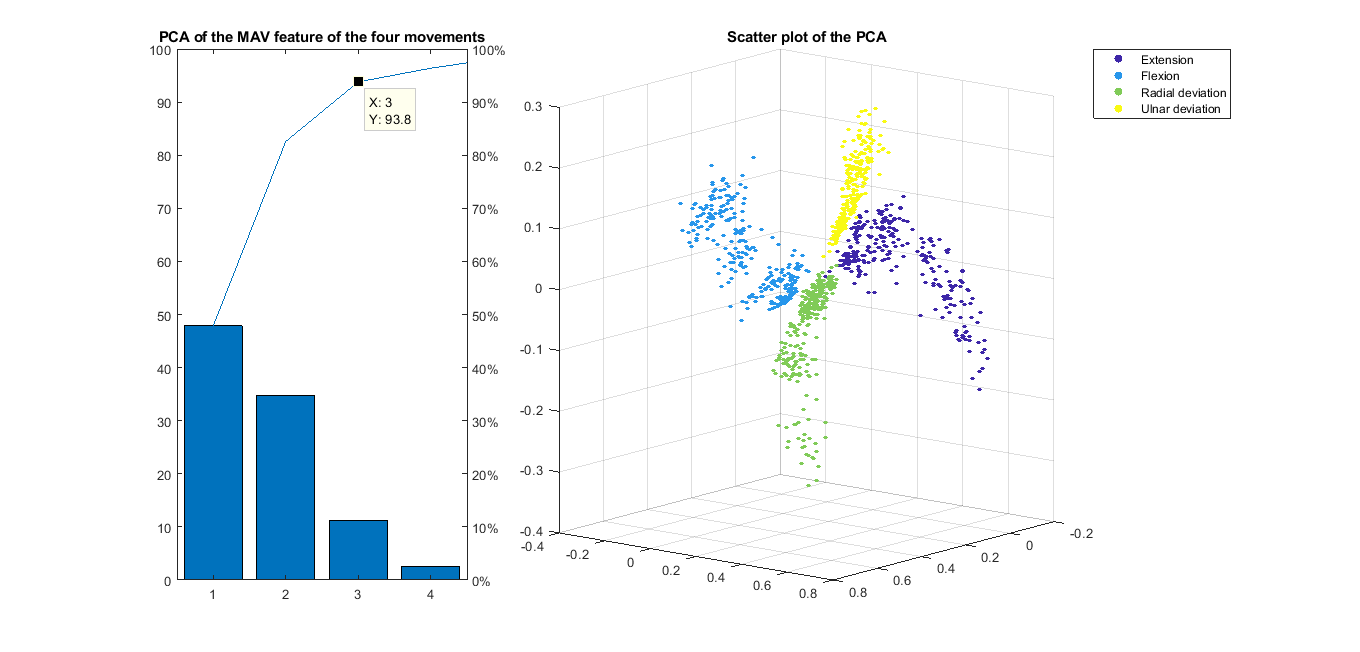
\includegraphics[scale=.27]{Figures/pcasubplotMAV}
	%\caption{Inductance of oscillation winding on amorphous
	%	magnetic core versus DC bias magnetic field}
	%\label{PCA_MVA}
	%\end{figure}
	

	
	\section{DISCUSSION}
	
		%discussion points
The present paper had as porpuose to study the performance of linear regression methods for myoelectric prostheses control taking in acount the limb position effect. Along the process different aspects have been exposed that are important to mention.\\
%subdivide in sections??
%Potential outliers were discoverd during this study. Even though the final results present that is possible to achieve simultaneous and proportional control using Myo armband, it had been shown that the sampling rate of this device could affect the acquisition of sEMG data. This could be due to the fact that sEMG signals  rate is between 10-500Hz, however the sampling rate of the Myoarmband is 200Hz, which casuses important information in raw data to be eliminated.
%Based on prevoius studies two different features were extracted in order to tran the regressors MAV and LogVar.
%A study by Hanhe \cite{hanhe2014} et al. showed that LogVar presented linear properties and outperformed the other different features extracted for that particular research. However the obtained results in our study illustrates that MAV performance outperformed the LogVar results. 
%Futhermore online results were not siginificant different depending on the limb position as other studies had shown for classification control scheme. This findings agree with a recently published study by Hwang et al. \cite{Hwang2017}. In their study different limb position were tested using Root Mean Square (RMS) as feature to train the regressors.
%During the results examination it was found that there is no correlation between the offline and online results. On the one hand the offline outcomes illustrates overfitting of the regression models. On the other hand the online test yielded robust control of the wrist movements performanced in the three different limb positions. This could be owing to the subjects$'$ ability to compensate for a poorer fitting model when visual feedback is provided.
%It have been proved that is possible to achieve simultaneous and proportional control in myoelectric prosthesis using linear regression techniques. 
%\begin{itemize}
	%\item inclusion of more subjects
%	\item sample rate of the myo armband - exclusion of test subjects
	%\item even though LogVar shows linearity in a previous study, it does not perform better in linear regression than a presumably non-linear feature
	%\item Both features does not show significant difference in control in different limb positions
%	\item Whatever the inclusion of IMU shows 
	
%	\item It is possible to use regression as control method to yield no significantly different performance in variations of limb positions
	%\item Use other regression methods and other features to analyse if it will result in better performance
	%\item why does the inclusion of IMU improve the performance
%	\item No connection between offline and online tests, which also is shown in previous studies
%	\item reasonable control can be archived when donning/doffing(we train the regressors with data, take of the myo armband, and do the testing with the myo armband placed slightly elsewhere)
	
%\end{itemize}
	\subsection{Offline and online training}
	Offline and online training was done for both MAV and LogVar without IMU data included, with a significant difference between the two features when testing with training data (p = 0.0044) but no difference when testing with new data (p = 0.1138). Overall it was found that there were no apparent correlation between offline and online testing. This could be caused by the subjects ability to adjust to a poor fitted model when given the visual feedback while performing the target test. This finding corresponds to the findings in other studies \cite{jiang2010}.
	
	\subsection{Comparison of features}
	In the results it was found that there was no significant difference between the performance of LogVar and MAV when it comes to the scores for the target test both with (p = 0.5637) and without (p = 0.0833) IMU data included. Based on previous studies showing LogVar as a feature with linear properties, it would be expected that this feature would perform better in a linear regression model, than a feature which to the authors knowledge has not been proven to be linear. On the contrary it was shown that a significantly higher number of targets was reached with a linear regression models based on the MAV feature with IMU included, compared to the LogVar regression model with IMU included (p = 0.0017). When IMU data wasn't included, there was no difference between the number of targets reached in the test (p = 1).
	
	Further studies within this field should consider examining other features, while studying the effect of combining several features in order to yield better performance independent of the limb position.
	
	\subsection{Inclusion of IMU data}
	The IMU data included in this study was based on a single accelerometer, where it was expected that the Myo band would give a similar output as long as the subjects were performing both training and testing from the same starting position. Inclusion of the IMU data was shown to yield the same results when it comes to the test score, with no significant difference for either MAV (p = 0.1779) or LogVar (p = 0.5637) when comparing regression models build with and without accelerometer inputs. It was found that the inclusion of the IMU data yielded significantly worse results for the LogVar regression model (p = 0.0016), while it led to a significant improvement of the MAV regression model (p = 0.0124) when examining the number of reached targets. The inclusion of IMU data could be a subject of further investigation, as the results might be improved by implementing a system capable of measuring the angles of the joints, in order to create a more versatile and usable regression model outside the clinical environment.  
	
	\subsection{Stability in limb positions}
	When excluding IMU data, there was no significant difference between the target score for either LogVar (p = 0.2359) or MAV (p = 0.8948) in the different limb positions, while there was a difference between the number of reached targets for MAV (0.0212) but no difference for LogVar (p = 0.4220). This outcome shows that both MAV and LogVar yields rather stable performance in different limb positions when used to create linear regression based control schemes.
	
	When including IMU data the MAV based regression model was shown to have a significant difference between the score of different limb positions (p = 0.0319), while LogVar did not show any difference (p = 0.4594). While the time taken to reach targets were shown to be different depending on limb positions when using MAV, the number of targets reached was improved, so that the number of reached targets with MAV were not shown to be significantly different (p = 0.2957). The LogVar feature based regression models were shown to have a difference between reached targets when using IMU data (p = 0.0037).
	
	Overall the LogVar regression models were observed as being the most unstable in the different limb positions when looking at the test subjects performance in the target test. This might be a result of the LogVar feature being based on the change of the signal, as this could lead to problems with crosstalk when the arm is not in a relaxed state. The MAV was observed as being more stable, with the subjects being able to create more controlled movements as well as having the possibility to adjust the position of the arrow when trying to get back to the middle of the test GUI. Based on the findings of this study, it would be recommended to examine features based on the amplitude rather than the variance in future studies within this area.
	
	\subsection{Limitations of the study}
	This study was based on data from 12 test subjects, where three had to be excluded. One subject was excluded due to misunderstanding the given instructions and thereby creating an unusable set of training and test data, which limited the control of the regression models giving him a mean score above 25 seconds per target and average number of reached targets below 10 for all tests.
	
	Two other subjects were excluded as the recorded intensities were not high enough to differ between the baseline and the intended movement. This caused the regression models to interpret the baseline in the target test as movements being performed at between 30\% and 70\% of the MVC.
	
	To improve the validity of the study more test subjects should be included in further studies within this field. Subjects with transradial amputations should also be taken into consideration if the regression based control schemes were to be considered for future use in myoelectric prosthetic devices. 
	
	Using the Myo band for data acquisition led to certain limitations in the sample rate, as the device is only capable of recording signals between 0 and 200Hz. This leads to the final signal being recorded between 0 and 100Hz, where everything above 100Hz is affected by aliasing. Along with frequency limitations, the Myo band restricted the number and placement of electrodes to eight channels placed at the same distance from the elbow, where it might be possible to yield better results with a different electrode placement and number. Further studies should implement regular EMG electrodes in order to obtain a more usable and clear signal, that represents the entire frequency band of EMG signals.
	
	
%	\begin{table}[h]
%		\caption{An Example of a Table}
%		\label{table_example}
%		\begin{center}
%			\begin{tabular}{|c||c|}
%				\hline
%				One & Two\\
%				\hline
%				Three & Four\\
%				\hline
%			\end{tabular}
%		\end{center}
%	\end{table}
	


	
	
	%Figure Labels: Use 8 point Times New Roman for Figure labels. Use words rather than symbols or abbreviations when writing Figure axis labels to avoid confusing the reader. As an example, write the quantity ÒMagnetizationÓ, or ÒMagnetization, MÓ, not just ÒMÓ. If including units in the label, present them within parentheses. Do not label axes only with units. In the example, write ÒMagnetization (A/m)Ó or ÒMagnetization {A[m(1)]}Ó, not just ÒA/mÓ. Do not label axes with a ratio of quantities and units. For example, write ÒTemperature (K)Ó, not ÒTemperature/K.Ó
	
	\section{CONCLUSIONS}
	
 		Linear regression methods were applied for the two different features extracted. We compared both performance, training the regressor with EMG data as well as a combination of EMG data and IMU data.
	
	\addtolength{\textheight}{-12cm}   % This command serves to balance the column lengths
	% on the last page of the document manually. It shortens
	% the textheight of the last page by a suitable amount.
	% This command does not take effect until the next page
	% so it should come on the page before the last. Make
	% sure that you do not shorten the textheight too much.
 		
	
	%%%%%%%%%%%%%%%%%%%%%%%%%%%%%%%%%%%%%%%%%%%%%%%%%%%%%%%%%%%%%%%%%%%%%%%%%%%%%%%%
	
	
	
	%%%%%%%%%%%%%%%%%%%%%%%%%%%%%%%%%%%%%%%%%%%%%%%%%%%%%%%%%%%%%%%%%%%%%%%%%%%%%%%%
	
	
	
	%%%%%%%%%%%%%%%%%%%%%%%%%%%%%%%%%%%%%%%%%%%%%%%%%%%%%%%%%%%%%%%%%%%%%%%%%%%%%%%%
	\section*{APPENDIX}
	
	Appendixes should appear before the acknowledgment.
	
	\section*{ACKNOWLEDGMENT}
	
	The preferred spelling of the word ÒacknowledgmentÓ in America is without an ÒeÓ after the ÒgÓ. Avoid the stilted expression, ÒOne of us (R. B. G.) thanks . . .Ó  Instead, try ÒR. B. G. thanksÓ. Put sponsor acknowledgments in the unnumbered footnote on the first page.
	
	
	
	%%%%%%%%%%%%%%%%%%%%%%%%%%%%%%%%%%%%%%%%%%%%%%%%%%%%%%%%%%%%%%%%%%%%%%%%%%%%%%%%
	
	References are important to the reader; therefore, each citation must be complete and correct. If at all possible, references should be commonly available publications.
	
	
	
	\begin{thebibliography}{99}
		
		\bibitem{c1} G. O. Young, ÒSynthetic structure of industrial plastics (Book style with paper title and editor),Ó 	in Plastics, 2nd ed. vol. 3, J. Peters, Ed.  New York: McGraw-Hill, 1964, pp. 15Ð64.
		\bibitem{c2} W.-K. Chen, Linear Networks and Systems (Book style).	Belmont, CA: Wadsworth, 1993, pp. 123Ð135.
		\bibitem{c3} H. Poor, An Introduction to Signal Detection and Estimation.   New York: Springer-Verlag, 1985, ch. 4.
		\bibitem{c4} B. Smith, ÒAn approach to graphs of linear forms (Unpublished work style),Ó unpublished.
		\bibitem{c5} E. H. Miller, ÒA note on reflector arrays (Periodical styleÑAccepted for publication),Ó IEEE Trans. Antennas Propagat., to be publised.
		\bibitem{c6} J. Wang, ÒFundamentals of erbium-doped fiber amplifiers arrays (Periodical styleÑSubmitted for publication),Ó IEEE J. Quantum Electron., submitted for publication.
		\bibitem{c7} C. J. Kaufman, Rocky Mountain Research Lab., Boulder, CO, private communication, May 1995.
		\bibitem{c8} Y. Yorozu, M. Hirano, K. Oka, and Y. Tagawa, ÒElectron spectroscopy studies on magneto-optical media and plastic substrate interfaces(Translation Journals style),Ó IEEE Transl. J. Magn.Jpn., vol. 2, Aug. 1987, pp. 740Ð741 [Dig. 9th Annu. Conf. Magnetics Japan, 1982, p. 301].
		\bibitem{c9} M. Young, The Techincal Writers Handbook.  Mill Valley, CA: University Science, 1989.
		\bibitem{c10} J. U. Duncombe, ÒInfrared navigationÑPart I: An assessment of feasibility (Periodical style),Ó IEEE Trans. Electron Devices, vol. ED-11, pp. 34Ð39, Jan. 1959.
		\bibitem{c11} S. Chen, B. Mulgrew, and P. M. Grant, ÒA clustering technique for digital communications channel equalization using radial basis function networks,Ó IEEE Trans. Neural Networks, vol. 4, pp. 570Ð578, July 1993.
		\bibitem{c12} R. W. Lucky, ÒAutomatic equalization for digital communication,Ó Bell Syst. Tech. J., vol. 44, no. 4, pp. 547Ð588, Apr. 1965.
		\bibitem{c13} S. P. Bingulac, ÒOn the compatibility of adaptive controllers (Published Conference Proceedings style),Ó in Proc. 4th Annu. Allerton Conf. Circuits and Systems Theory, New York, 1994, pp. 8Ð16.
		\bibitem{c14} G. R. Faulhaber, ÒDesign of service systems with priority reservation,Ó in Conf. Rec. 1995 IEEE Int. Conf. Communications, pp. 3Ð8.
		\bibitem{c15} W. D. Doyle, ÒMagnetization reversal in films with biaxial anisotropy,Ó in 1987 Proc. INTERMAG Conf., pp. 2.2-1Ð2.2-6.
		\bibitem{c16} G. W. Juette and L. E. Zeffanella, ÒRadio noise currents n short sections on bundle conductors (Presented Conference Paper style),Ó presented at the IEEE Summer power Meeting, Dallas, TX, June 22Ð27, 1990, Paper 90 SM 690-0 PWRS.
		\bibitem{c17} J. G. Kreifeldt, ÒAn analysis of surface-detected EMG as an amplitude-modulated noise,Ó presented at the 1989 Int. Conf. Medicine and Biological Engineering, Chicago, IL.
		\bibitem{c18} J. Williams, ÒNarrow-band analyzer (Thesis or Dissertation style),Ó Ph.D. dissertation, Dept. Elect. Eng., Harvard Univ., Cambridge, MA, 1993. 
		\bibitem{c19} N. Kawasaki, ÒParametric study of thermal and chemical nonequilibrium nozzle flow,Ó M.S. thesis, Dept. Electron. Eng., Osaka Univ., Osaka, Japan, 1993.
		\bibitem{c20} J. P. Wilkinson, ÒNonlinear resonant circuit devices (Patent style),Ó U.S. Patent 3 624 12, July 16, 1990. 
		
		
		
		
		
		
	\end{thebibliography}
	
	
	
	
\end{document}